% !TEX encoding = UTF-8
% !TEX TS-program = pdflatex
% !TEX root = ../tesi.tex

%**************************************************************
\chapter{Resoconto dello stage}
\label{cap:resoconto-stage}
%**************************************************************

\intro{In questo capitolo verranno descritte le attività svolte durante lo stage. Per ogni attività si cercherà di descrivere il problema affrontato, le scelte effettuate ed i test svolti.}\\

\section{Pianificazione}
La prima attività svolta, in realtà ancora prima dell'inizio dello stage stesso, è stata quella di pianificare il lavoro da svolgere. Tale pianificazione è stata concordata tra il tutor aziendale e il sottoscritto, ed è esposta nella sezione \ref{sec:vincoli-temporali} a pagina \pageref{sec:vincoli-temporali} di questo documento.\\
Tale pianificazione, però, è stata "aggiustata" (ma mai stravolta) in base a quanto svolto settimana per settimana, decidendo di dedicare più o meno ore ad una determinata attività.\\
Al termine di ogni settimana, periodo coincidente con il raggiungimento di un obiettivo, infine, è stato deciso che avrei dovuto redarre una breve relazione, con lo scopo di documentare il lavoro svolto. Tali relazioni, inoltre, sono servite come materiale ausiliario per la presentazione delle nuove funzionalità sviluppate al proponente. Infine, terminati tutti gli obiettivi e in caso di approvazione da parte del tutor e del proponente, avrei dovuto trasferire il lavoro svolto dall'ambiente di sviluppo a quello di produzione.

\section{Funzionamento e struttura del \bookingEngine}
Appena iniziato lo stage, mi sono subito dedicato all'analisi della struttura di CrociereRegalo, grazie anche (soprattutto all'inizio) all'aiuto del mio tutor. 
\subsection{Funzionalità}
CrociereRegalo è un motore di ricerca di crociere. Permette di trovare una determinata crociera utilizzando dei filtri di ricerca per area geografica (ad esempio Caraibi, Mediterraneo, Nord Europa), per data di partenza con granularità mensile (ad esempio Settembre 2018), per intervalli di durata (da 1-6, 7-8, 9-12 o più di 12 giorni) e per compagnia di crociera (ad esempio MSC Crociere). Per capire bene il suo funzionamento è stato necessario apprendere alcuni termini tecnici affini all'ambiente croceristico, come :
\begin{itemize}
	\item \textbf{Itinerario}: definisce il percorso che fa una crociera (ad esempio "Barcellona, Ajaccio, Civitavecchia, Barcellona"). Nell'arco di un periodo di tempo vi possono essere molteplici crociere percorrenti un singolo itinerario. Ogni itinerario è identificato da un codice che lo contraddistingue univocamente, e la durata dell'itinerario è una proprietà intrinseca (ovvero, all'interno di una compagnia di crociera, non esistono due itinerari che svolgono lo stesso percorso mettendoci tempi diversi). Ciascun itinerario ha 0 o più partenze nell'arco di un anno;
	\item \textbf{Cabina}: é una stanza di una nave da crociera. Esistono varie categorie di cabina, differenziate in base alla grandezza, al posizionamento (ad esempio le cabine interne alla nave, senza quindi finestre, che sono quelle più economiche). Quando si effettua una prenotazione, non viene prenotato un posto letto ma viene prenotata un'intera cabina;
	\item \textbf{Opzione}: consiste nel blocco del prezzo di una cabina per un periodo di tempo che varia in base al fornitore, ma che di solito si attesta tra le 24 e le 72 ore. Tale prezzo infatti, analogamente per quanto avviene con i biglietti aerei, aumenta all'aumentare delle prenotazioni (quindi al passare del tempo).

\end{itemize}
Premesso ciò, CrociereRegalo permette di selezionare un itinerario, vederne le partenze, categorie di cabina disponibili e prezzi e poi prenotare od opzionare una cabina. 

\subsection{OTA e DataExchange}
Mi è stato spiegato che il \bookingEngine, in realtà, era spezzato in due parti dipendenti l'una dall'altra: \textbf{OTA} (disponibile all'indirizzo \url{https://www.crociereregalo.it}) e \textbf{DataExchange} (disponibile all'indirizzo \url{https://data.crociereregalo.it}). L'idea alla base di questa divisione è che la parte \textit{OTA} rappresenti il sito web vero e proprio, con il quale l'internauta si affaccia, mentre la parte \textit{DataExchange} serva per l'interazione tra \textit{OTA} e \glspl{webservice} dei vari fornitori (dove per fornitori si intendono le varie compagnie di crociera). 

\subsection{Interazione tra OTA e DataExchange}
\textit{OTA} e \textit{DataExchange} sono sì dipendenti l'uno dall'altro, ma hanno due database separati. Questo, fondamentalmente, avviene perchè i dati provenienti da i vari fornitori hanno formati diversi, che devono quindi essere uniformati per poter essere processati secondo una logica più indipendente possibile. Il compito del \textit{DataExchange} è proprio questo: interrogare i \glspl{webservice} dei vari fornitori, ricevere i dati, elaborarli, uniformarli e passarli ad \textit{OTA}.\\
Premesso ciò, vi sono due possibili interazioni tra \textit{OTA} e \textit{DataExchange}
\begin{itemize}
	\item Interazione \textbf{schedulata}, che avviene circa 3 volte al giorno, il cui compito è sincronizzare i cataloghi (chiamati anche \textit{flatfile}) dei vari fornitori per rendere disponibili le (eventuali) modifiche alla parte \textit{OTA} del \bookingEngine. \\Quando un visitatore del sito CrociereRegalo cerca una crociera, tale ricerca avviene interrogando i cataloghi presenti nel database della parte \textit{OTA}, senza quindi interrogare i \glspl{webservice} delle compagnie di crociera (per motivi di prestazione dovuti all'ingente mole di dati da elaborare). I cataloghi, quindi, vengono scaricati nel DataExchange, elaborati (uniformati) e poi sincronizzati con il database di OTA; la procedura di sincronizzazione viene chiamata \textbf{Integrazione}. L'integrazione avviene attraverso l'invocazione (grazie allo scheduler di \textit{Windows Server}) che, grazie ad una chiamata \textit{HTTP} ad una particolare pagina del DataExchange, invoca la procedura di integrazione dati.
	\begin{figure}[!h] 
		\centering 
		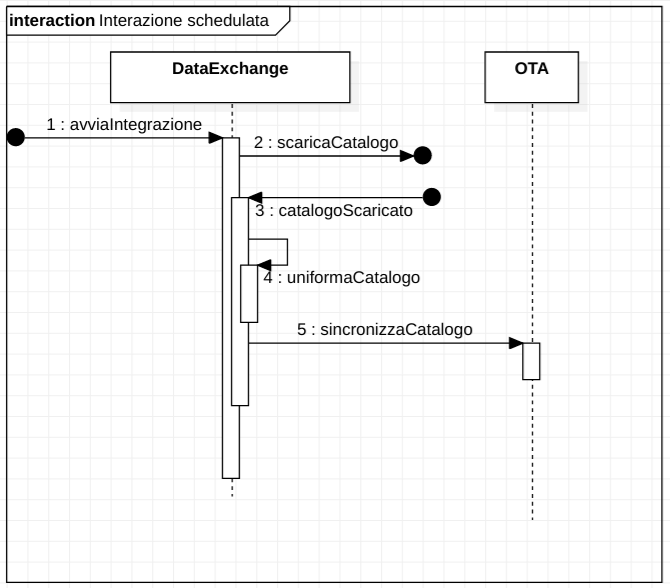
\includegraphics[width=.75\columnwidth]{attivita/interazione_schedulata} 
		\caption{Schema dell'integrazione schedulata appena descritta.}
	\end{figure}
	\item Interazione \textbf{real-time}, che avviene durante tutto il flusso di prenotazione di una cabina (che analizzerò in seguito). Tale flusso deve per forza disporre di dati aggiornati in tempo reale, altrimenti potrebbero verificarsi problemi in fase di prenotazione (come la prenotazione di una cabina non più disponibile). L'interazione in tempo reale avviene attraverso delle chiamate \textit{HTTP} (ajax) effettuate nel momento del bisogno dall'\textit{OTA} al \textit{DataExchange}, attraverso lo scambio di dati in formato \textit{JSON}.
	\begin{figure}[!h] 
		\centering 
		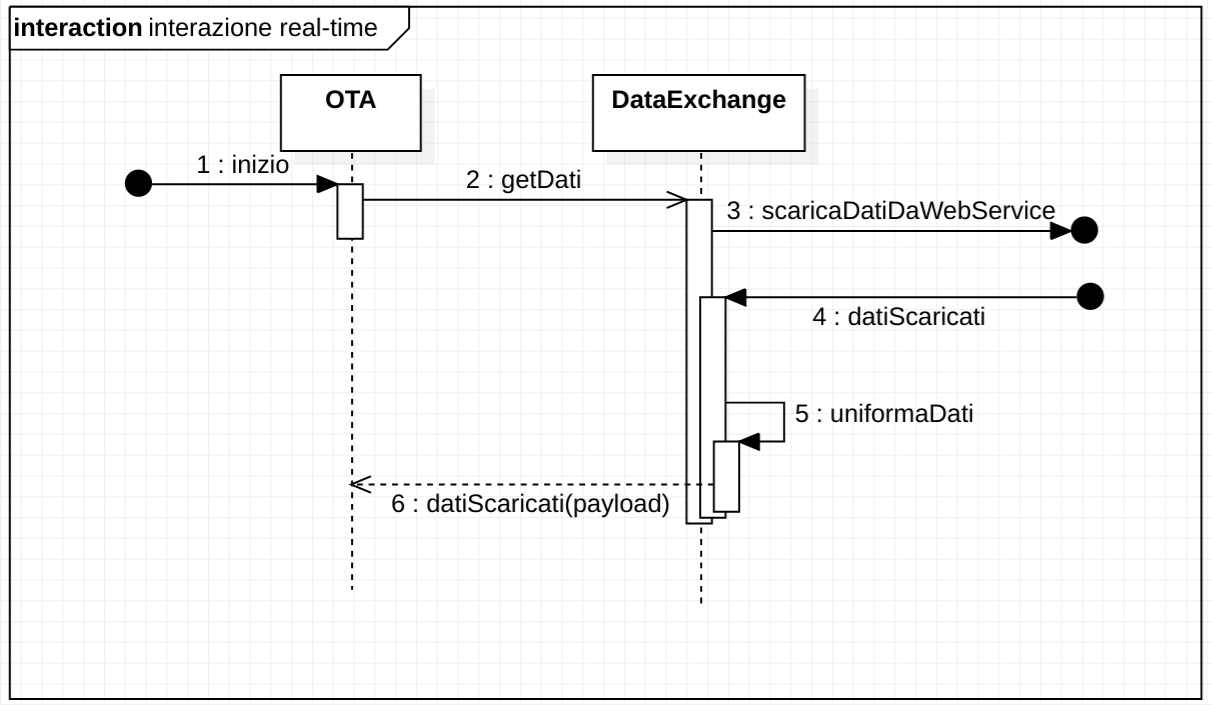
\includegraphics[width=.75\columnwidth]{attivita/interazione_realtime} 
		\caption{Schema dell'integrazione in tempo reale appena descritta.}
	\end{figure}
\end{itemize}

\subsection{Flusso di prenotazione}
\label{section:flusso-prenotazione}
Quando il visitatore, in seguito alla ricerca, apre i dettagli di una partenza, viene data la possibilità di poter avviare la procedura (flusso) di prenotazione, che si avvale dell'interazione real-time tra \textit{OTA} e \textit{DataExchange} si compone nei seguenti punti:
\begin{enumerate}
	\item \textit{categoryAvailability}: vengono elencati i gruppi (categorie) di cabine effettivamente disponibili (o un messaggio di errore in caso non vi siano più posti prenotabili) tenendo conto del numero di passeggeri inseriti (banalmente, se si selezionano 4 passeggeri, vengono mostrati le categorie di cabine nelle quali vi è presente almeno una quadrupla) e dell'età di tali passeggeri (per il calcolo preciso della tariffa, in quanto un minore paga meno di un adulto);
	\item \textit{cabinAvailability}: una volta selezionato una categoria di cabine, vengono mostrate tutte le cabine (una per una) ancora disponibili, raggruppate in base al ponte della nave in cui si trovano;
	\item \textit{categoryItem}: vengono elencati tutti i servizi extra (e relativi prezzi) disponibili in aggiunta a quelli già inclusi nel prezzo della cabina, e viene data la possibilità di selezionarli per aggiungerli alla prenotazione;
	\item \textit{requestPricing}: viene mostrato il prezzo finale (preso dal \gls{webservice} del fornitore) della prenotazione, tenendo conto di quanto selezionato negli step precedenti. Tale prezzo include anche le tasse portuali ed eventuali oneri aggiuntivi;
	\item \textit{requestBooking}: viene effettuata una prenotazione od un'opzione di quanto selezionato negli step del flusso precedenti. Nel caso di prenotazione, viene anche gestito il pagamento (tramite \gls{api} fornite dal consorzio \textit{Triveneto Bassilichi}).
	\item \textit{requestBookingInformation}: viene mostrato il riepilogo di ciò acquistato, con la possibilità di saldare quanto ancora dovuto (nel caso la prenotazione ammetta il versamento di un acconto).
\end{enumerate}

\subsection{Struttura del codice}
Sia \textit{OTA} che \textit{DataExchange} sono realizzati usando il framework \textit{Codeigniter}. Questo implica che applicano a PHP il paradigma \textit{Object-oriented} (orientato agli oggetti) associato al design pattern \gls{mvc}. Entrambi i progetti, dunque, presentano tre tipologie di classi:
\begin{itemize}
	\item \textbf{Model}, che estendono la classe base \textit{CI\_Model}, i quali sono la chiave di accesso ai dati dell'applicazione. Si è deciso di realizzare un \textit{model} per ogni tabella presente nel database;
	\item \textbf{View}, che generano il codice HTML di ogni pagina (o porzione di essa). Alle \textit{view} é possibile passare delle variabili in modo da rendere dinamico il loro contenuto.
	\item \textbf{Controller}, che estendono la classe base \textit{CI\_Controller} e istanziano le \textit{view} popolandole con i dati provenienti dai \textit{model}. La particolarità di queste classi è che i loro metodi pubblici si possono chiamare direttamente tramite URL. Codeigniter, infatti, implementa un meccanismo (grazie al \textit{magic method \_\_call}) per il quale é possibile chiamare un metodo pubblico \textit{a} di una classe controller \textit{C} semplicemente recandosi all'url \textit{nomedelsito.dominio/C/a} (ad esempio \textit{crociereregalo.it/C/a}). Tale meccanismo risulta molto utile nella realizzazione di \gls{api} e nella creazione di \textit{URL} user-friendly (quindi più leggibili)
\end{itemize} 
Codeigniter, inoltre, presenta un modulo personalizzato per interagire con il database, che supporta funzionalità come il \textit{log delle query} (in pratica è possibile sapere l'ultima query eseguita, molto utile in caso di debug), meccanismi di \textit{query builder} (creazione assitita di query), \textit{query parametrizzate}, gestione delle transazioni ecc.

\section{Ottimizzazione delle performance del database}
\subsection{Il problema}
Il sito CrociereRegalo soffriva di un grande problema: la velocità di caricamento delle pagine. Tale lentezza era dovuta principalmente all'elevato numero di query complesse presenti in ogni pagina, ciascuna delle quali aveva dei tempi di esecuzione nell'ordine dei secondi che, complessivamente, facevano sì che il tempo di caricamento di alcune pagine (in primis quella di visualizzazione dei risultati di una ricerca) lambisse pericolosamente il minuto.
\subsection{La soluzione trovata}
Dopo un'attenta analisi del database, é emerso che molte tabelle non avevano una corretta struttura. In particolare, su alcune non vi era definita alcuna chiave primaria, mentre in generale non erano presenti chiavi esterne ed indici. Sono quindi state definite chiavi esterne e primarie per tutte le tabelle, mentre per la creazione di indici ci si è affidati all'analisi delle principali query grazie allo strumento \textit{Database Tuning Engine Advisor} integrato nella suite di \textit{SQL Server}. Vengono ora riportati due esempi di analisi svolta e di risultati ottenuti.
\subsubsection{Query di ricerca}

\begin{lstlisting}
SELECT distinct TOP 100 l.Supplier, l.NameIT, l.Description, l.Logo, il.ShipCode,il.SailingLengthDays, il.ItineraryCode, po1.Code as PortoPartenzaCode ,po1.Name as PortoPartenza, po2.Name as PortoArrivo, po2.Code as PortoArrivoCode, min(il.SailingDate) as MinSailingDate, min(p.BestPrice) as BestPrice,it.GraphicsUrl,sp.Name as ShipName 
FROM Cruises_ItineraryList il inner join Cruises_Lines l on il.Supplier= l.Supplier inner join Cruises_Ports po1 on (po1.Code = il.DepartingPort and po1.Supplier = il.Supplier ) inner join Cruises_Ports po2 on (po2.Code = il.EndPort and po2.Supplier = il.Supplier) inner join Cruises_Ship sp on (sp.Supplier=il.Supplier and sp.Code = il.ShipCode) inner join Cruises_Prices p on (p.Supplier=il.Supplier and p.CruiseId = il.CruiseID and p.CruiseCategoryAvailable=1) inner join Cruises_Itinerary it on (it.Supplier=il.Supplier and il.ItineraryCode = it.Code) 
WHERE il.Supplier=1 AND il.AvailabilityStatusCode= 'AV' AND BestPrice > 0 
GROUP By l.Supplier, l.NameIT, l.Description, l.Logo, il.ShipCode,il.SailingLengthDays, il.ItineraryCode, po1.Code, po2.Code, po1.Name, po2.Name , sp.ImgUrl,it.GraphicsUrl,sp.Name order by MinSailingDate,PortoArrivo,ItineraryCode
\end{lstlisting}
Questa é una delle query (la più esterna) che viene usata nel caso di ricerca di un itinerario filtrandolo per fornitore (in questo caso MSC Crociere). Il problema di questa interrogazione, oltre alla lunghezza, è l'elevato numero di JOIN tra tabelle aventi un ingente quantitativo di dati, nello specifico:
\begin{itemize}
	\item Cruises\_Prices: 424 780 righe
	\item Cruises\_ItineraryList: 8 092 righe
	\item Cruises\_Ports: 4 187 righe
	\item Cruises\_Itinerary: 2 985 righe
\end{itemize}

Tali tabelle erano per lo più sprovviste di indici, pertanto le operazioni di JOIN risultavano molto costose. Come risultato si otteneva un tempo di esecuzione, nel server di produzione in assenza di sovraccarichi, variabile tra 23 e 25 secondi. Grazie al tool \textit{Database Tuning Engine Advisor} sono stati creati dei nuovi indici, precisamente su tutte le colonne coinvolte nelle clausole di JOIN. Questo ha portato un ingente riduzione nei tempi di esecuzione della query, che sono arrivati a sfiorare i 2 secondi. Vi è stato, quindi, un miglioramento di ben almeno 21 secondi (circa il 91\%) nel tempo di esecuzione della query e di conseguenza nel \gls{tempodirisposta} della pagina web incaricata di elaborare e visualizzare i risultati della ricerca.\\
\begin{figure}[!h] 
	\centering 
	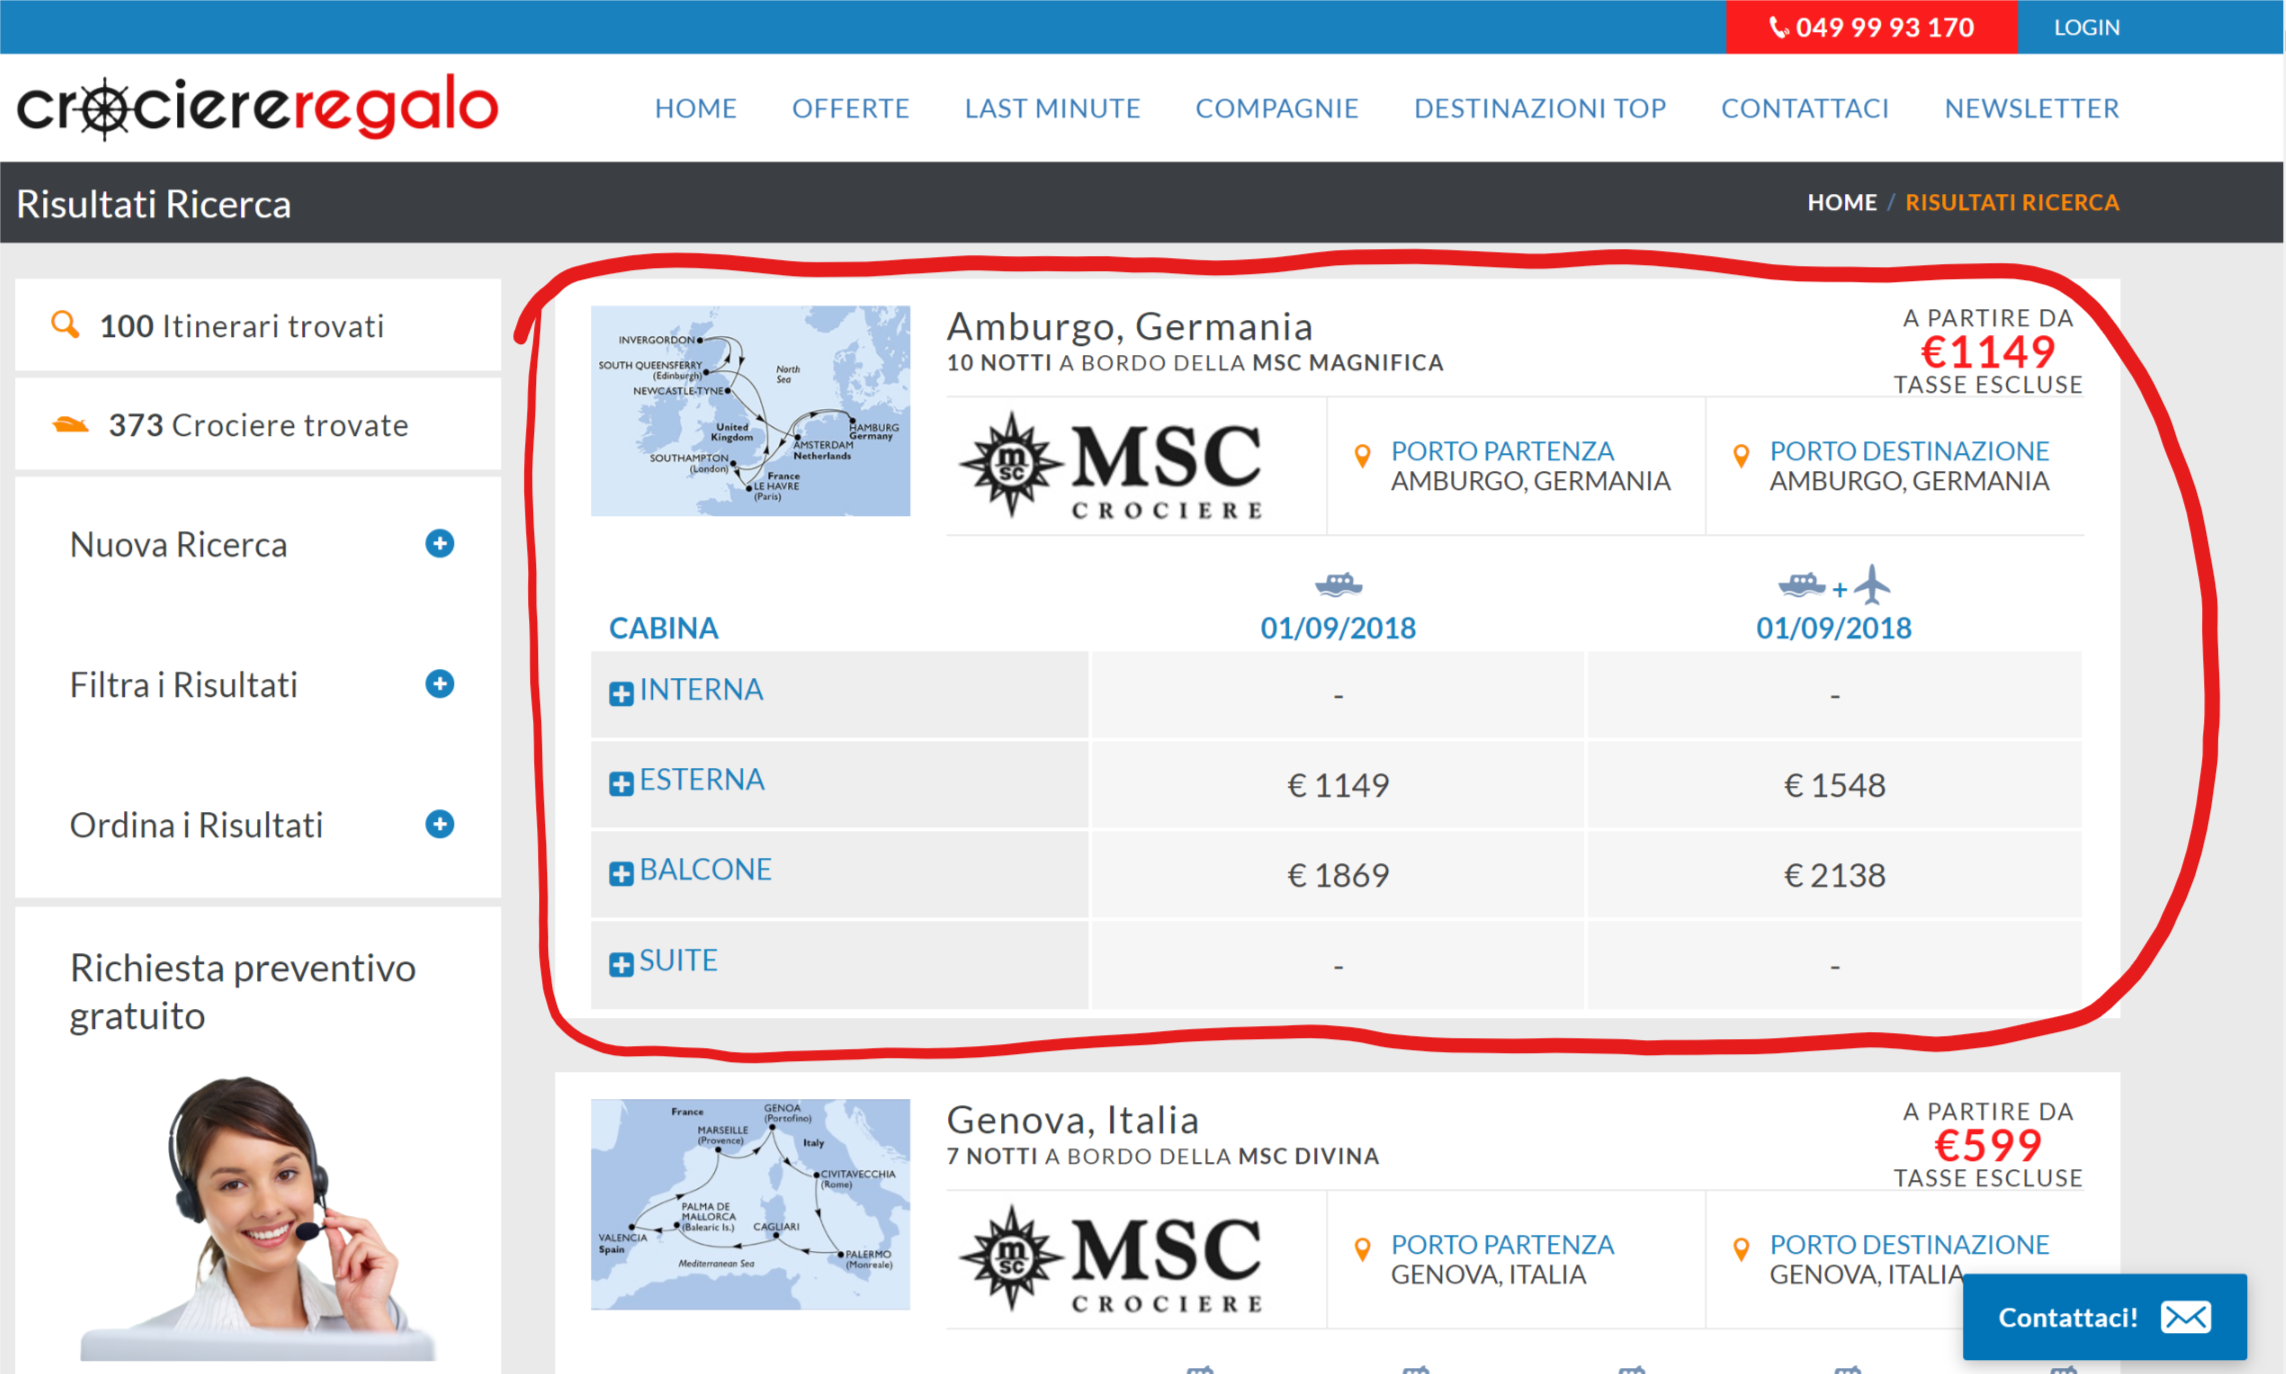
\includegraphics[width=1\columnwidth]{attivita/risultato_ricerca} 
	\caption{Esempio di utilizzo del risultato della query sopra menzionata.}
\end{figure}

\subsubsection{Query dei last minute}
In homepage vi è una sezione che visualizza tutte le offerte \textit{last minute} (ovvero crociere prossime alla partenza aventi ancora posti disponibili a prezzo scontato) presenti nel database. Queste ultime vengono inserite a mano dai dipendenti di \textit{Primarete}, ma sono collegate a crociere effettivamente presenti. La query sottostante restituisce tali offerte.
\begin{lstlisting}
SELECT distinct top 4 l.Logo,l.NameIT as SupplierName,il.Supplier,il.CruiseID,il.ShipCode, il.ItineraryCode,il.DepartingPort,il.EndPort,il.SailingDate,il.ReturnDate,il.SailingLengthDays as NightNumber,po.Name as Partenza,po2.Name as Arrivo,s.foto,sp.ImgUrl,min(p.BestPrice) as BestPrice FROM Cruises_ItineraryList il join Cruises_Prices p on il.CruiseID = p.CruiseId join Cruises_Ports po on (il.DepartingPort = po.Code and po.Supplier=il.supplier) join Cruises_Ports po2 on (il.EndPort = po2.Code and po2.Supplier=il.supplier) join Cruises_Ship sp on (sp.Code=il.ShipCode and sp.Supplier=il.Supplier) join Cruises_Lines l on (l.Supplier=il.Supplier) left join Cruises_Banner AS b ON b.tipo = 'nave' AND b.riferimento = CONCAT(il.Supplier,'-',il.ShipCode) INNER JOIN Cruises_Banner_Slide AS s ON b.id = s.banner AND s.nome='nave'
 WHERE SailingDate BETWEEN '2018-09-09' and '2018-10-09' and AvailabilityStatusCode='AV' and il.supplier = 2 and po.Supplier= 2 and po2.Supplier=2 and p.BestPrice>0 group by l.Logo,l.NameIT,il.Supplier,il.CruiseID,il.ShipCode, il.ItineraryCode,il.DepartingPort,il.EndPort,il.SailingDate,il.ReturnDate,il.SailingLengthDays,po.Name ,po2.Name ,s.foto,sp.ImgUrl
\end{lstlisting}
Anche qua, il numero di JOIN su tabelle aventi ingenti quantità di dati rende il tempo di esecuzione della query molto elevato in caso il database non sia sufficientemente ottimizzato. Grazie alle ottimizzazioni suggerite dal tool \textit{Database Tuning Engine Advisor}, si è avuto un miglioramento del tempo di esecuzione indicativamente dell'83\%, che è passato da 3 secondi a 0.5. Tale miglioramento si è riflettuto anche nelle performance della homepage, che ha visto una netta diminuzione del tempo medio di risposta.
\begin{figure}[!h] 
	\centering 
	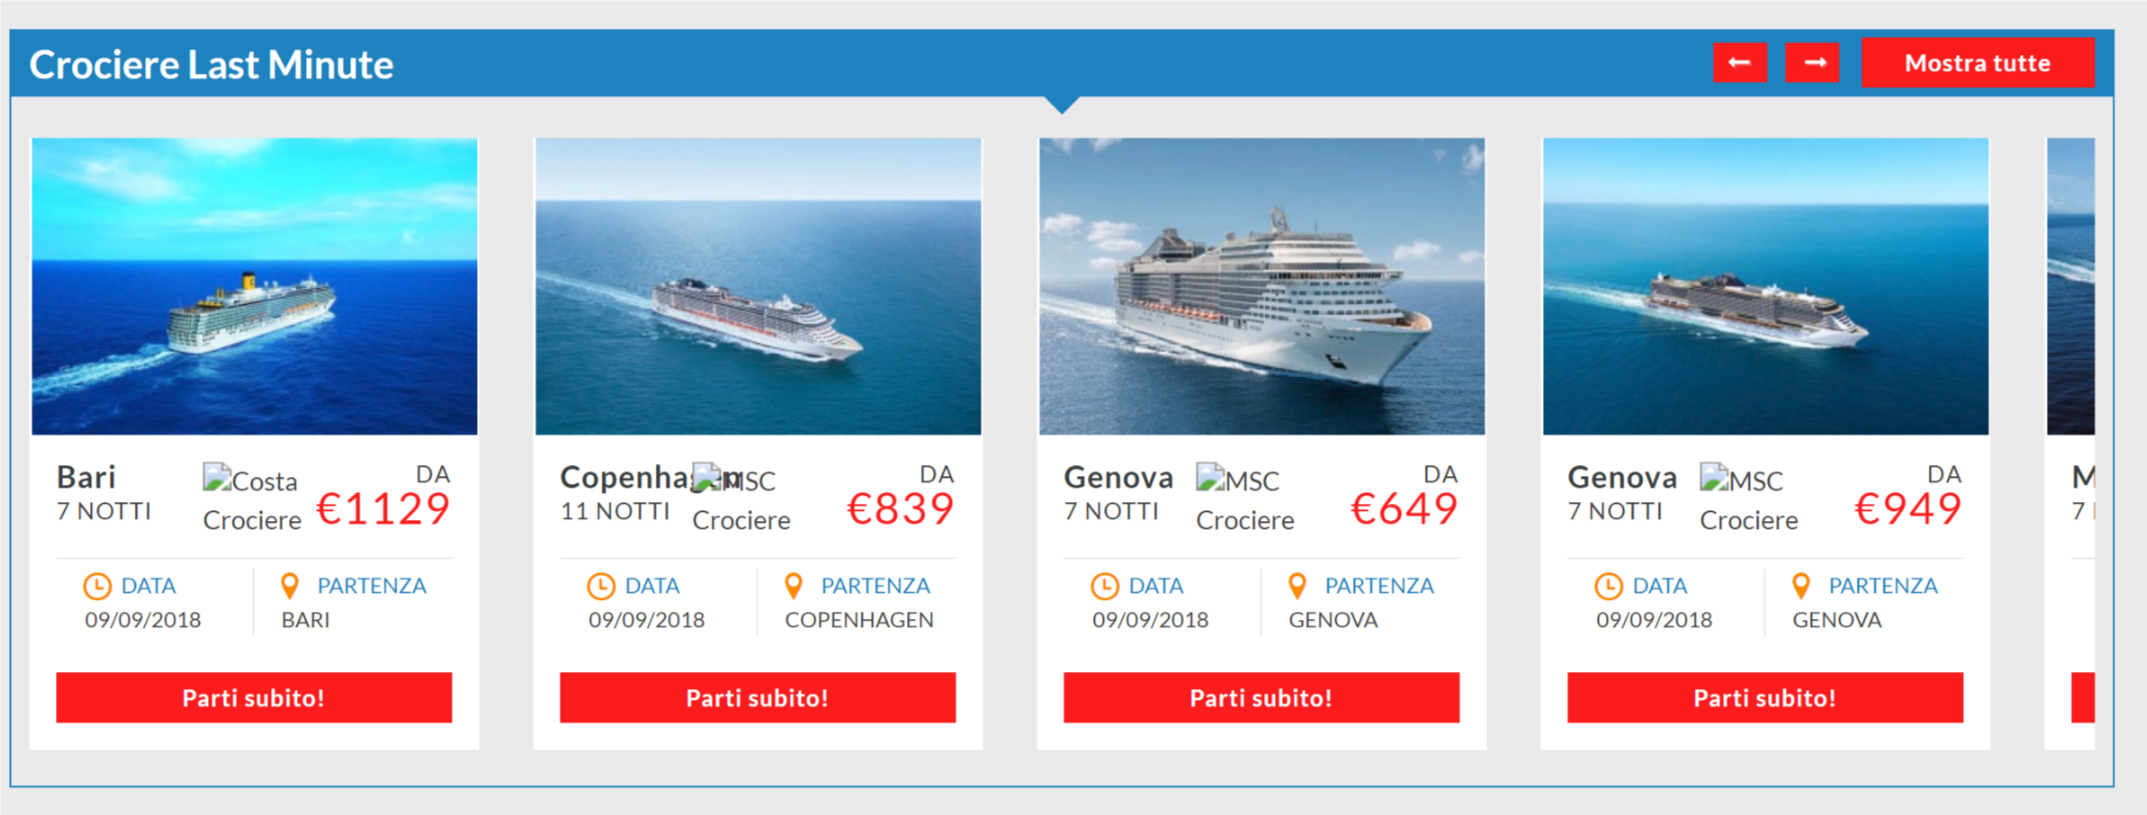
\includegraphics[width=1\columnwidth]{attivita/last_minute} 
	\caption{Esempio di utilizzo del risultato della query sopra menzionata.}
\end{figure}

\subsection{Conclusioni}
Al termine delle ottimizzazioni, sono stati ottenuti buoni risultati (il \gls{tempodirisposta} del sito è diminuito di almeno il 50\%), ma non abbastanza per rendere il sito reattivo ed equiparabile in termini di velocità ai competitor. Si è deciso quindi di esplorare nuove soluzioni.

\section{Cache delle query}
\subsection{Il problema}
Se é vero che, al termine degli interventi sulla struttura del database descritti nella sezione precedente, le prestazioni delle interrogazioni erano migliorate molto, è anche vero che il sito non aveva raggiunto livelli di prestazioni ottimali. Infatti alcune pagine avevano ancora un \gls{tempodirisposta} molto elevato. Prendendo come esempio la pagina del sito più utilizzata, ovvero quella di visualizzazione dei risultati di una ricerca, essa è passata da un \gls{tempodirisposta} tra i 45 e i 60 secondi ad un \gls{tempodirisposta} tra i 15 e i 20 secondi, comunque troppo per le aspettative di un internauta medio: basti pensare che il principale competitor (\url{www.logitravel.it}) ha un \gls{tempodirisposta} che si attesta attorno al secondo e mezzo (10 volte meno) per la stessa funzionalità.

\subsection{La soluzione}
La soluzione trovata a tale problema nasce dalla seguente considerazione: é possibile prevedere quando cambia la maggior parte dei dati presenti nel database e utilizzati per le query più lente. Infatti dati inerenti a navi, itinerari, cabine, prezzi e disponibilità vengono rinnovati ad ogni integrazione, che è un'operazione schedulata 4 volte al giorno, ad orari noti. Osservando inoltre che la stessa query sugli stessi dati presenta gli stessi risultati, si è giunti alla conclusione che l'implementazione di un meccanismo di caching delle query permetta di ottimizzare velocità del sito e carico del server.\\
Il meccanismo progettato ha il seguente funzionamento:
\begin{itemize}
	\item La query viene eseguita la prima volta ed il suo risultato viene salvato nella cache;
	\item Quando la query viene eseguita ancora, invece di interrogare il database viene letto il contenuto della cache;
	\item Ad ogni integrazione dati la cache viene svuotata, perchè i dati presenti in essa non riflettono più il nuovo contenuto delle tabelle del database;
	\item Al termine di ogni integrazione, vengono effettuate delle richieste \textit{CURL} alle pagine più utilizzate del sito, in modo tale che la cache venga ricreata.
\end{itemize}
Si è deciso di affidare la gestione della cache a \textit{Codeigniter}, che offre già questa funzionalità. Il modulo di gestione del database di \textit{Codeigniter}, infatti, fornisce già i seguenti metodi:
\begin{itemize}
	\item \textit{cache\_on}, che permette di abilitare la cache;
	\item \textit{cache\_off}, che permette di disabilitare la cache;
	\item \textit{cache\_delete}, che permette di cancellare la cache di una singola pagina (passata come parametro);
	\item \textit{cache\_delete\_all}, che permette di cancellare tutto il contenuto della cache.
\end{itemize}
Combinando l'uso di \textit{cache\_on} e \textit{cache\_off}, si può anche disabilitare la cache per determinate query, che magari operano su dati più "volatili" e aventi minor quantità. \\In generale, comunque, \textit{Codeigniter} salva i risultati delle varie query in dei file di cache (aventi come nome l'hash della query a cui tale file si riferisce) suddivisi per cartelle in base all'url che le ha generate.
\begin{figure}[!h] 
	\centering 
	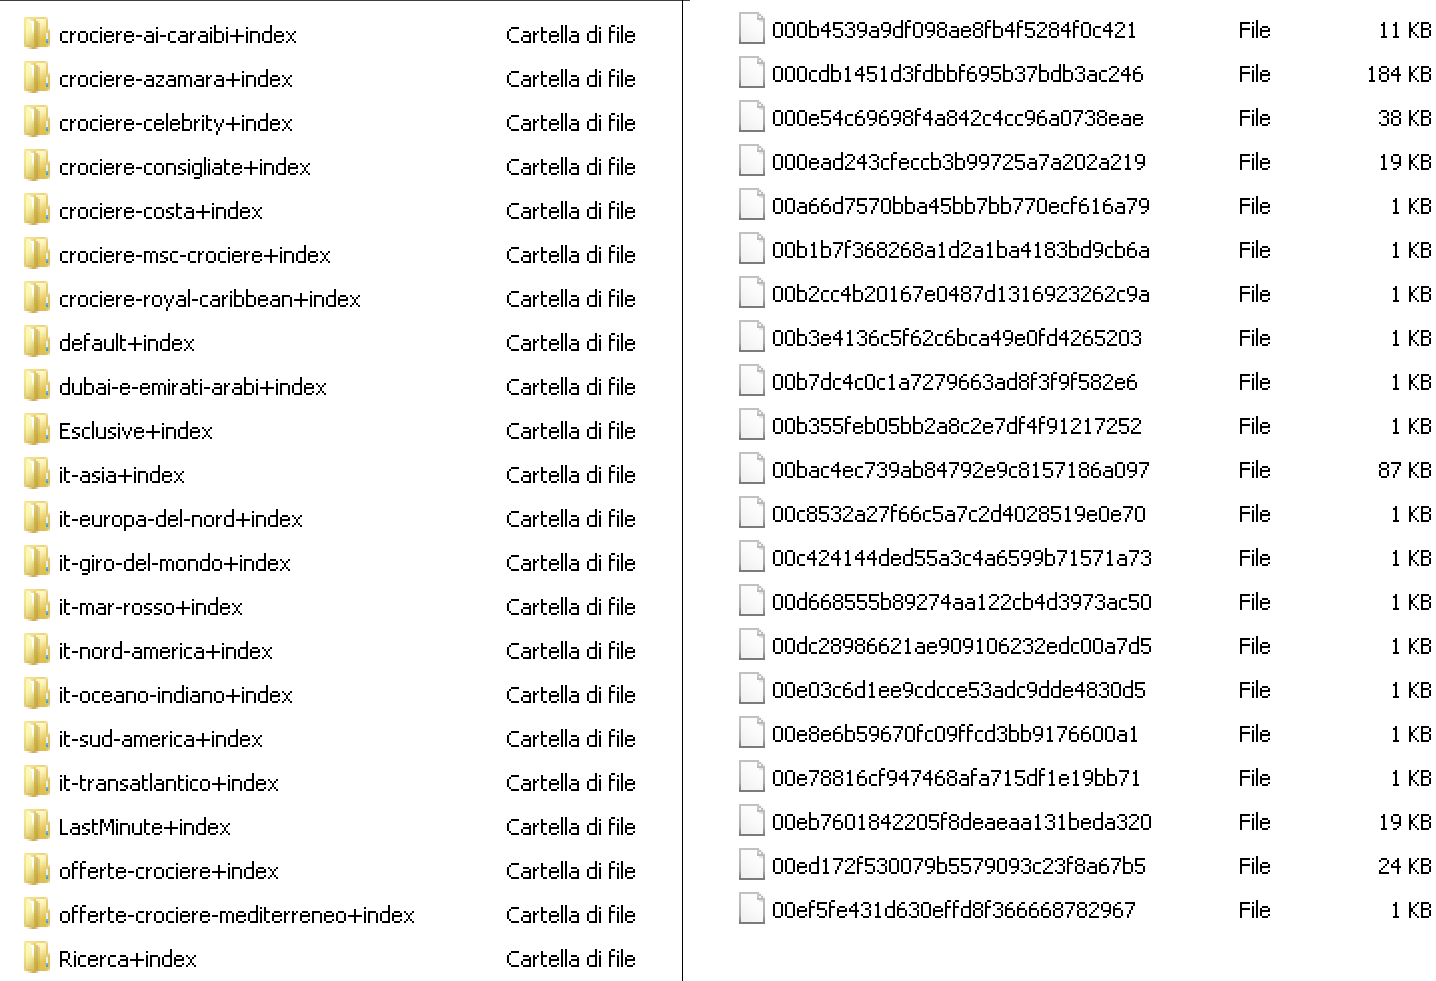
\includegraphics[width=1\columnwidth]{attivita/cache_codeigniter} 
	\caption{Struttura di cartelle e file di cache in esse contenuti.}
\end{figure}
Grazie a \textit{cache\_delete} sarebbe possibile cancellare la cache solo di alcune pagine, ma è stato preferito non utilizzare tale funzione in quanto avrebbe aumentato inutilmente la complessità della soluzione.

\subsection{Risultati}
L'implementazione della cache ha giovato molto al \bookingEngine. Basti pensare che ora la pagina di visualizzazione dei risultati ricerca è giunta ad avere un tempo di risposta medio attorno ai 3 secondi, ovvero ora è l'80\% più veloce di prima, ma soprattutto è paragonabile al tempo di risposta dei competitor. Il tempo di risposta della homepage, inoltre, è arrivata a toccare i 500 millisecondi, dai circa 3 secondi prima di implementare la cache.\\
Tra ottimizzazione del database e cache, comunque, sono stati fatti ingenti miglioramenti alle prestazioni, che riassumo nella tabella sottostante, prendendo come esempio la pagina principale e quella di visualizzazione dei risultati della ricerca (che, per brevità, chiamerò soltanto "ricerca").\\

\begin{center}
	\def\arraystretch{1.5}
	\begin{tabular}{ | l | l | l | l |}
		\hline
		\textbf{Pagina} & \textbf{Senza ottimizzazioni} & \textbf{Con DB ottimizzato} & \textbf{Con cache} \\ \hline
		Homepage & 7 secondi & 3 secondi & 0.5 secondi.  \\
		\hline
		Ricerca & 45-60 secondi & 15-20 secondi & 3 secondi.  \\
		\hline
	\end{tabular}
\end{center}

\newpage
\section{Integrazione delle tariffe vuoto per pieno}
\subsection{Il problema}
Dopo aver preso effettivamente confidenza con il database, mi è stato chiesto come secondo lavoro di creare un sistema che permettesse di inserire nel flusso di prenotazione anche tariffe vuoto per pieno. Precisamente, tale sistema avrebbe dovuto avere le seguenti caratteristiche:
\begin{enumerate}
	\item Permettere di inserire nel sistema gli acquisti di vuoti pieno effettuati da \textit{Primarete} tramite upload di appositi file;
	\item Permettere di differenziare i prezzi in base al soggetto a cui si sta vendendo;
	\item Permettere di prenotare e pagare una cabina con tariffa vuoto per pieno.
\end{enumerate}

\subsubsection{Inserimento degli acquisti nel sistema}
Il sistema avrebbe dovuto prevedere una funzionalità di "carico" delle tariffe. In fase di acquisto dei vuoti pieno da parte di \textit{Primarete}, il fornitore (ovvero la compagnia di crociera) rilascia un file riepilogativo contenente il dettaglio di quanto acquistato. Tali informazioni avrebbero dovuto potersi caricare in modo assistito nel sistema, che avrebbe dovuto poi inserirle nel flusso di prenotazione.\\
Il problema principale è stato che il file ritornato da ciascun fornitore aveva (e ha tuttora) il proprio formato dati, quindi si sarebbe dovuto creare un importatore per ogni fornitore. Inoltre, anche la tipologia di dati presente in ciascun file poteva differire: ad esempio, per riferirsi all'età di ogni passeggero, alcuni fornitori utilizzano l'età ed altri la data di nascita. Il sistema avrebbe dunque dovuto uniformare i dati caricati.

\subsubsection{Differenziazione dei prezzi}
CrociereRegalo è un \bookingEngine utilizzato per vendite sia B2C (cioè verso clienti finali) sia B2B (cioè verso altre agenzie). Queste ultime, in base agli accordi commerciali che hanno con \textit{Primarete}, appartengono a determinati \textit{listini}, ovvero hanno diritto a commissioni/tariffe più o meno agevolate.\\Il sistema, quindi, avrebbe dovuto poter differenziare i prezzi di vendita delle cabine in base al listino di appartenenza dell'acquirente (un acquirente non appartenente a nessun listino sarebbe stato identificato al pari di una vendita B2C).

\subsubsection{Inserimento della tariffa nel flusso di prenotazione}
Il \bookingEngine avrebbe dovuto permettere di visualizzare i prezzi delle cabine soggette a tariffe vuoto per pieno nei risultati di ricerca. Inoltre, avrebbe dovuto essere possibile poter prenotare e conseguentemente pagare tali cabine.\\La disponibilità delle stesse, quindi, si sarebbe dovuta aggiornare (decrementare) automaticamente.

\subsection{La soluzione}
\subsubsection{Inserimento degli acquisti nel sistema}
Affinché fosse possibile inserire gli acquisti nel sistema, è stata realizzata una nuova pagina nel pannello di amministrazione del \bookingEngine, accessibile solo tramite l'inserimento di username e password. In tale pagina viene visualizzato un riepilogo dei vuoti pieno caricati con la possibilità, per ognuno di essi, di avere il dettaglio delle cabine vendute e di quelle ancora disponibili. È stato inoltre inserito un tasto che apre una finestra di dialogo all'interno della quale viene data la possibilità di caricare nuovi vuoti pieno, andando quindi a "rifornire" il "magazzino". In base al fornitore selezionato nella finestra di dialogo è possibile: 
\begin{itemize}
	\item Caricare il file di riepilogo di quanto acquistato fornito dalla compagnia, in caso di fornitore \textbf{Costa} o \textbf{MSC}. Il primo fornisce un file con estensione \textit{.xls} mentre il secondo un file con estensione \textit{.csv}
	\begin{figure}[!h] 
		\centering 
		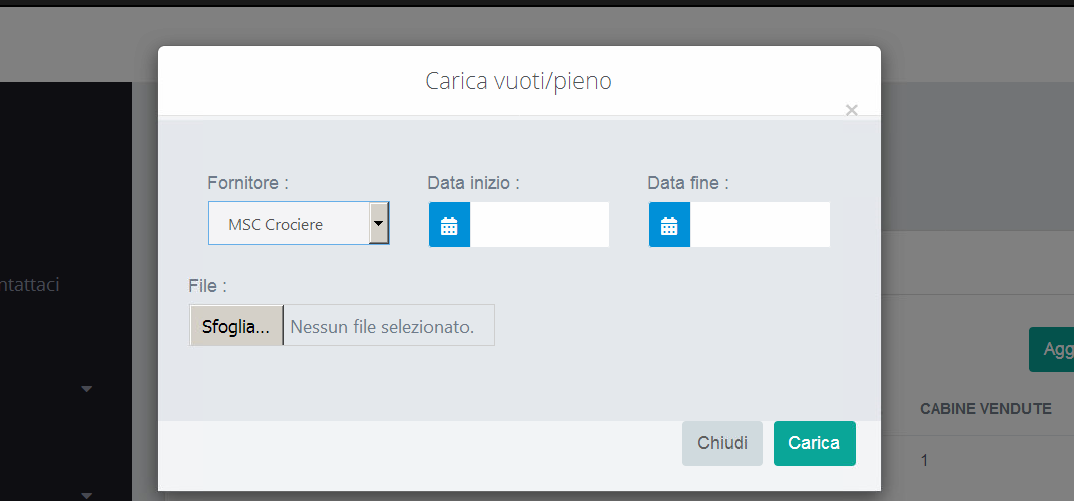
\includegraphics[width=.8\columnwidth]{attivita/vuotopieno_msc} 
		\caption{Schermata di caricamento del vuoto pieno MSC e Costa.}
	\end{figure}
	\item Inserire a mano i dettagli del vuoto pieno che si intende caricare nel caso di fornitore \textbf{Royal Caribbean}, \textbf{Celebrity} o \textbf{Azamara}. Essi infatti forniscono il file di riepilogo di quanto acquistato in formato \textit{.pdf}, che è molto difficile da interpretare.
	\begin{figure}[!h] 
		\centering 
		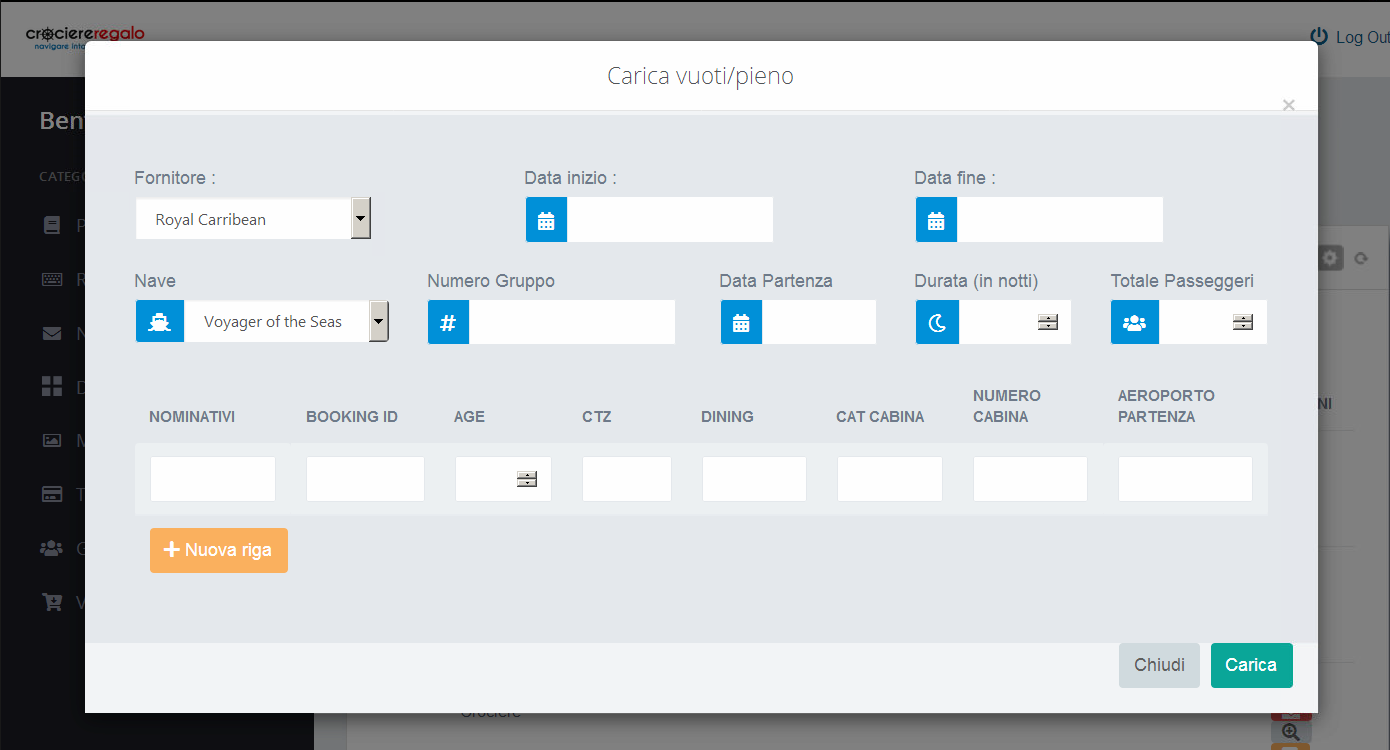
\includegraphics[width=.8\columnwidth]{attivita/vuotopieno_royal} 
		\caption{Schermata di caricamento del vuoto pieno Royal/Celebrity/Azamara.}
	\end{figure}
\end{itemize}
In ogni caso, é stato deciso che per ciascun vuoto pieno si sarebbero memorizzate le seguenti informazioni:
\begin{itemize}
	\item Il \textbf{fornitore}, ovvero MSC, Costa, Royal Caribbean, Celebrity o Azamara;
	\item Il \textbf{groupID}, ovvero un identificatore univoco per ciascun fornitore del vuoto pieno acquistato;
	\item Il \textbf{cruiseID}, ovvero un identificatore univoco per ciascun fornitore della crociera a cui tale vuoto pieno si riferisce;
	\item La \textbf{data di partenza} della crociera;
	\item La \textbf{lunghezza} (in numero di notti) della crociera;
	\item Il \textbf{numero di posti} (ovvero la capienza massima di persone) totali in quel vuoto pieno;
	\item Il \textbf{numero di cabine} totali di quel vuoto pieno,
	\item La \textbf{data di inizio} e la \textbf{data di fine} validità della tariffa, in modo che sia possibile venderla solo in determinati periodi/intervalli. Ciò significa che, ad esempio, se la data di inizio viene impostata al 20 agosto 2018 e la data di fine al 30 settembre 2018, in caso di una ricerca fatta prima del 20 agosto 2018 o dopo il 30 settembre 2018, la tariffa non comparirà tra i risultati.
\end{itemize}
Per memorizzare queste informazioni è stata creata una nuova tabella in database denominata \textbf{Cruises\_Inventory}, avente come campi \textit{Id} (chiave primaria auto incrementante), \textit{Supplier} (fornitore, chiave esterna che si riferisce a \textit{Cruises\_Lines}, tabella dove sono memorizzati tutti i fornitori), \textit{GroupID}, \textit{CruiseID}, \textit{DepartureDate} (data di partenza della crociera), \textit{Length} (lunghezza in notti della crociera), \textit{N\_Pax} (numero di posti totali), \textit{N\_Cab} (numero di cabine totali), \textit{Data\_Inizio} e \textit{Data\_Fine}.\\
\\
Oltre alle informazioni generali relative a ciascun vuoto pieno, è stato necessario memorizzarne anche il contenuto in dettaglio, in termini di cabine acquistate (e quindi da rivendere). Si è deciso di creare la tabella \textbf{Cruises\_InventoryDetail} avente i seguenti campi:
\begin{itemize}
	\item \textbf{Id}, chiave primaria auto incrementante;
	\item \textbf{Cruises\_Inventory}, chiave esterna collegata all'\textit{Id} dell'omonima tabella \textit{Cruises\_Inventory}, che serve per collegare ogni riga del dettaglio al vuoto pieno corrispondente;
	\item \textbf{Cruises\_PricesID}, chiave esterna collegata all'\textit{Id} di \textit{Cruises\_Prices}, tabella il cui scopo verrà analizzato nel dettaglio nella sezione successiva;
	\item \textbf{Cabin}, numero di cabina (univoco nel dominio del fornitore) a cui la riga corrente si sta riferendo;
	\item \textbf{BookId}, numero di prenotazione del fornitore della cabina a cui la riga corrente si sta riferendo;
	\item \textbf{Category}, categoria della cabina corrente.
\end{itemize}
Per gestire il caricamento dei vuoti pieno nel sistema sono state realizzate tre classi \textit{parser} (una per MSC, una per Costa e una per il trio Royal-Celebrity-Azamara)in grado di interpretare dei dati in input e renderli compatibili con la struttura delle tabelle \textit{Cruises\_Inventory} e \textit{Cruises\_InventoryDetail}. Queste tre classi, \textit{MSCParser}, \textit{CostaParser} e \textit{RoyalParser} implementano tutte l'interfaccia \textbf{ParserInterface}, che ha i seguenti metodi astratti:
\begin{center}
	\def\arraystretch{1.5}
	\begin{tabularx}{\columnwidth}{XX}
		\hline
		\textbf{Metodo} & \textbf{Descrizione} \\ \hline
		+ getCruiseID() : string & Ritorna il CruiseID corrispondente al vuoto pieno considerato\\
		\hline
		+ getGroupID() : string & Ritorna il GroupID corrispondente al vuoto pieno considerato\\
		\hline
		+ getDepartureDate() : string & Ritorna la data di partenza corrispondente al vuoto pieno considerato, in formato "Y-m-d" (esempio 2018-09-27).\\
		\hline
		+ getLength() : int & Ritorna la lunghezza (in numero di notti) corrispondente al vuoto pieno considerato.\\
		\hline
		+ getNPax() : int & Ritorna la capienza totale (in numero di persone) corrispondente al vuoto pieno considerato.\\
		\hline
		+ getNCab() : int & Ritorna la capienza totale (in numero di cabine) corrispondente al vuoto pieno considerato.\\
		\hline
		+ popolaDettaglioTabella() : array & Ritorna un array che, per ciascuna riga del vuoto pieno, associa a ciascun campo della tabella \textit{Cruises\_InventoryDetail} il relativo valore.\\
		\hline
	\end{tabularx}
\end{center}
È stata poi creata una nuova classe, \textbf{Cruises\_Inventory}, "figlia" di \textit{CI\_Model} (classe base dei modelli di Codeigniter), che si occupa principalmente del caricamento del vuoto pieno nel database, avvalendosi dei parser prima elencati. Di preciso, ha i seguenti metodi:
\begin{center}
	\def\arraystretch{1.5}
	\begin{longtable}{ >{\raggedright}p{5.5cm} p{6.8cm}} 
		\hline
		\textbf{Metodo} & \textbf{Descrizione} \\ \hline
		+ validId(id:int) : boolean & Ritorna \textit{true} se il parametro passato è un valore presente nella colonna "Id" della tabella \textit{Cruises\_Inventory}\\
		\hline
		+ loadFromFile (supplier: int, fileContent: string, dataInizio: Date, dataFine: Date) : void & In base al fornitore passato come parametro (\textit{supplier}), carica il contenuto del vuoto pieno (presente in \textit{fileContent}) nel database, avvalendosi del parser associato al fornitore.\\
		\hline
		- loadRoyalInput (supplier: int, content: array) : boolean & Carica il vuoto pieno Royal/Celebrity/Azamara (in base al valore della variabile \textit{supplier}) leggendo il contenuto dall'array associativo \textit{content} ed elaborandolo grazie al parser \textit{RoyalParser}.\\
		\hline
		- loadCostaFile (fileContent: string) : boolean & Carica il vuoto pieno Costa nel database; \textit{fileContent} rappresenta il contenuto del file del vuoto pieno caricato, che verrà elaborato dal parser \textit{CostaParser}.\\
		\hline
		- loadMSCFile (fileContent: string) : boolean & Carica il vuoto pieno MSC nel database; \textit{fileContent} rappresenta il contenuto del file del vuoto pieno caricato, che verrà elaborato dal parser \textit{MSCParser}.\\
		\hline
		- saveParsedFile(parser: ParserInterface, supplier: int) : boolean & Metodo che viene chiamato da \textit{loadRoyalInput}, \textit{loadCostaFile}, \textit{loadMSCFile}; serve a popolare la tabella \textit{Cruises\_InventoryDetail} e la tabella \textit{Cruises\_Prices}.\\
		\hline
	\end{longtable}
\end{center}
La gestione del pannello di amministrazione è affidata ad un unico \textit{controller}, chiamato \textbf{Back}. In questa classe è stato aggiunto un metodo chiamato \textit{caricaVuotoPieno} che prende l'input dal frontend e lo passa al metodo \textit{loadFromFile} della classe \textit{Cruises\_Inventory} appena descritta, che si occuperà dell'elaborazione e della restituzione del risultato della stessa sotto forma di JSON.

\subsubsection{Differenziazione dei prezzi}
I prezzi di ogni cabina presente nel sistema risiedono nella tabella \textit{Cruises\_Prices}. Tale tabella permette di conoscere il prezzo di ogni categoria di cabina (per ogni combinazione di età dei passeggeri tollerata dal sistema) per ogni \gls{tariffa} disponibile. Il problema è che \textit{Cruises\_Prices} viene svuotata e ripopolata ad ogni integrazione: per questo motivo si è deciso di separare la gestione dei prezzi delle cabine soggette a tariffa vuoto per pieno in una nuova tabella, che è stata chiamata \textit{Cruises\_InventoryPrices}. Di preciso:
\begin{itemize}
	\item Nella tabella \textit{Cruises\_Prices} è stata inserita una nuova colonna di tipo intero, \textbf{Manuale}, che indica se la riga si sta riferendo ad una tariffa passata dal fornitore o presa da un vuoto pieno. Quando viene fatta un'integrazione, vengono eliminate solo le righe aventi valore di tale colonna pari a 0, in modo da non perdere le informazioni relative al vuoto pieno;
	\item È stata creata la tabella \textbf{Cruises\_InventoryPrices}, avente i seguenti campi:
		\begin{itemize}
			\item \textit{Id}, identificatore univoco della riga;
			\item \textit{Cruises\_Inventory}, chiave esterna che si riferisce al campo \textit{Id} di \textit{Cruises\_Inventory} e specifica il vuoto pieno di appartenenza di tale riga;
			\item \textit{Listino}, chiave esterna di \textit{Cruises\_Listini}, tabella appena creata che verrà descrittà nel prossimo paragrafo. In caso di valori NULL, il listino si intende essere \textit{B2C}, ovvero vendita al dettaglio;
			\item \textit{Categoria}, che rappresenta la categoria della cabina a cui ci si sta riferendo;
			\item \textit{Cabina}, che rappresenta il numero di cabina a cui ci si sta riferendo;
			\item \textit{BookId}, che indica il codice di prenotazione del fornitore collegato alla cabina a cui ci si sta riferendo;
			\item Un campo per ogni combinazione di prezzi tollerata dal sistema, ovvero \textit{Price1Adult, Price2Adult, Price3Adult, Price4Adult, Price1Adult1Junior, Price1Adult1Junior1Child, Price2Adult1Child, Price2Adult2Child,Price2Adult1Child, Price2Adult2Junior, Price2Adult1Junior1Child};
			\item \textit{Commissione}, che quantifica la commissione spettante all'agenzia viaggi collegata al listino specificato, in caso il campo \textit{Listino} non sia NULL.
		\end{itemize}
\end{itemize}
La tabella \textbf{Cruises\_Listini} menzionata precedentemente è stata creata per poter gestire tutti i listini da collegare alle varie agenzie viaggi. Tale tabella presenta due campi, \textit{Id} e \textit{Nome}, usati appunto per definire il listino stesso. \\
Nella tabella \textit{Cruises\_Utenti}, che raccoglie tutte le agenzie viaggio che possono accedere alla modalità di acquisto B2B, è stato aggiunto il campo \textit{Listino}, chiave esterna di \textit{Cruises\_Listini}, in modo da associare ogni agenzia registrata ad un listino, in base agli accordi presi con \textit{Primarete}. \\ \\
Per l'interazione con la tabella \textit{Cruises\_InventoryPrices} è stato creato un nuovo model avente lo stesso nome della tabella, con i seguenti metodi: 
\begin{center}
	\def\arraystretch{1.5}
	\begin{longtable}{ >{\raggedright}p{5.5cm} p{6.8cm}} 
		\hline
		\textbf{Metodo} & \textbf{Descrizione} \\ \hline
		+ getColonnePrezzi() : array & Ritorna un array contentente la lista di tutte le combinazioni di prezzi tollerata dal sistema. Questo metodo è stato scritto per rendere poi dinamico l'inserimento dei prezzi in questa tabella, ovvero in caso si voglia aggiungere un nuovo campo non presente (ad esempio \textit{Price6Adult}), sarà sufficiente aggiungerlo come colonna della tabella, e interfaccia grafica e query di inserimento si adatteranno automaticamente. \\
		\hline
		+ tentaAggiornamentoPrezzi (tabella: array, inventoryId: int) : void & Metodo che prova ad aggiornare i prezzi nel caso di caricamento di un vuoto pieno contenente cabine già presenti nel sistema.\\
		\hline
		+ salvaPrezzi (input: array) : boolean & Metodo che salva i prezzi di ogni cabina, per ogni listino, presenti nel parametro \textit{input}. Ritorna "true" in caso di successo, "false" altrimenti.\\
		\hline
		+ modificaPrezzi (input: array) : boolean & Metodo che modifica i prezzi di ogni cabina, per ogni listino, presenti nel parametro \textit{input}. Ritorna "true" in caso di successo, "false" altrimenti.\\
		\hline
	\end{longtable}
\end{center}
È stato inoltre creato un metodo \textit{salvaPrezzi} nel controller \textit{Back}, che si limita ad invocare il metodo \textit{salvaPrezzi} del model \textit{Cruises\_InventoryPrices} con i parametri passati tramite POST.\\
A livello frontend, si è fatto in modo che, al termine del caricamento del vuoto pieno, si venga reindirizzati ad una pagina di inserimento prezzi, che permette appunto di specificare ogni combinazione di prezzo tollerata dal sistema per ogni categoria di cabina per ciascun listino. 
	\begin{figure}[!h] 
	\centering 
	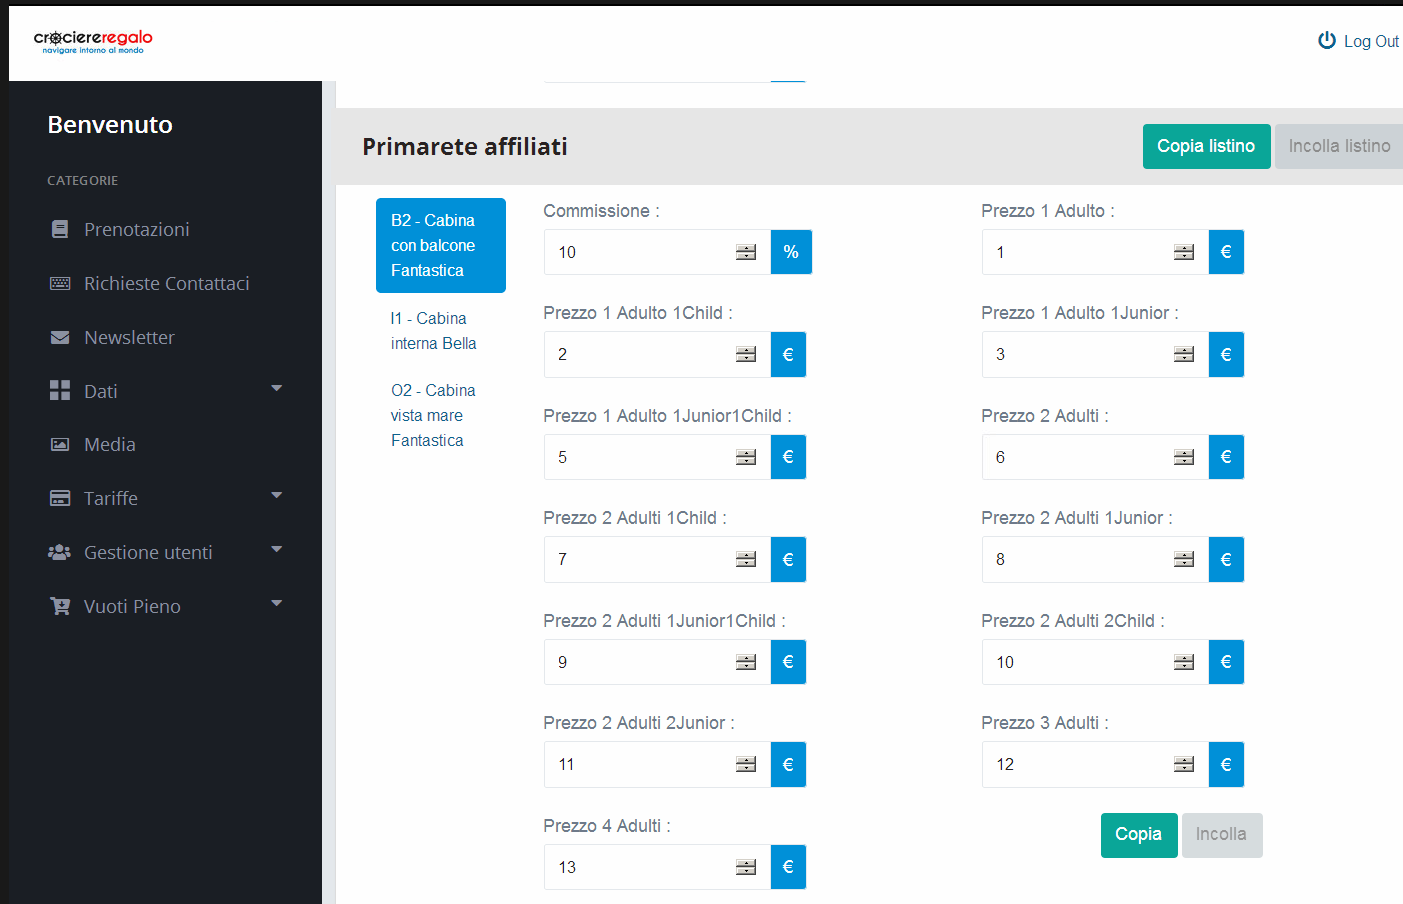
\includegraphics[width=1\columnwidth]{attivita/vuotopieno_prezzi} 
	\caption{Schermata di inserimento dei prezzi di un vuoto pieno.}
\end{figure}\\
I prezzi poi vengono salvati tramite una chiamata AJAX che invoca il metodo \textit{salvaPrezzi} del controller \textit{Back} precedentemente descritto.

\subsubsection{Inserimento della tariffa nel flusso di prenotazione}
Come già accennato nella \hyperref[section:flusso-prenotazione]{sezione \ref*{section:flusso-prenotazione}}, il flusso di prenotazione si compone di 6 step, a ciascuno dei quali corrisponde un metodo nel controller \textbf{WS\_Cruises} del \textit{dataExchange}. Questi 6 metodi venivano (e vengono tuttora) chiamati tramite richieste AJAX dal frontend e al loro interno chiamavano l'omologo metodo in grado di interfacciarsi con i \gls{webservice} del fornitore considerato.\\
Sono stati quindi creati i seguenti metodi:
\begin{center}
	\def\arraystretch{1.5}
	\begin{longtable}{ >{\raggedright}p{5.5cm} p{6.8cm}} 
		\hline
		\textbf{Metodo} & \textbf{Descrizione} \\ \hline
		+ Inventory\_categoryAvailabilty (inout wsResult:array) : void & Concatena al risultato eventualmente restituito dai \gls{webservice} del fornitore le categorie di cabine, se presenti, aventi tariffa vuoto per pieno. Il codice della tariffa restituita (dato che servirà alle successive funzioni) è "INVENTORY".\\
		\hline
		+ Inventory\_cabinAvailabilty () : array & Legge dal database (facendo delle query su Cruises\_Inventory, Cruises\_InventoryDetail e Cruises\_InventoryPrices) e restituisce le singole cabine disponibili, compreso il prezzo, secondo i qualificatori che legge dal payload della richiesta, quali numero ed età dei passeggeri, cruiseID considerato, categoria delle cabine di cui si vuole controllare la disponibilità e listino di appartenenza dell'utente.\\
		\hline
		+ Inventory\_requestPricing () : array & Calcola un preventivo in base ai parametri passati nel payload della richiesta, ovvero fornitore, cruiseID, numero della cabina, dati anagrafici dei passeggeri.\\
		\hline
		+ Inventory\_requestBooking () : string & Prenota la cabina passata come parametro nel payload della richiesta e ritorna il bookingID (identificativo della prenotazione) corrispondente.\\
		\hline
		+ Inventory \_requestBookingInformation (bookId: string) : array & Dato il bookId passato come parametro, restituisce tutti i dettagli inerenti alla prenotazione. \\
		\hline
	\end{longtable}
\end{center}
Il primo metodo del flusso, \textit{categoryAvailability}, in base al valore del parametro \textit{supplier} (letto dal payload della richiesta), invocava i metodi \textit{MSC\_categoryAvailability} o \textit{Costa\_categoryAvailability}, che interrogano i rispettivi \glspl{webservice}. È stato sufficiente quindi che il nuovo metodo creato \textit{Inventory\_categoryAvailabilty} venisse invocato da \textit{categoryAvailabilty} a prescindere dal \textit{supplier}, concatenando all'output dei metodi \textit{MSC\_categoryAvailability} o \textit{Costa\_categoryAvailability} le categorie di cabine eventualmente disponibili con tariffa vuoto per pieno.\\
Nei metodi \textit{cabinAvailability}, \textit{requestPricing}, \textit{requestBooking} e \textit{requestBookingInformation}, è stata introdotta un'istruzione condizionale che, in base al \textbf{fareCode} (codice della tariffa) passato come parametro, decida se invocare l'omologo metodo che legga dal database delle tariffe vuoto per pieno (in caso di fareCode = "INVENTORY") o dai \glspl{webservice} del fornitore.\\
Al frontend, infine, non è stato necessario fare alcuna modifica.
\newpage
\section{Royal}